\section{Model Hyperparameters}
\label{appendix:hypers}
In this section, we detail the hyperparameters for our models, each tuned for specific environments and design configurations. The tuning process utilized Bayesian optimization via the wandb sweep tool \citep{wandb}. The optimization objective was chosen to maximize both the performance score achieved by the model and the efficiency in the number of actions utilized. The objective function was structured as follows:

\[
n_a/N + \text{final\_normalized\_return},
\]

where $n_a$ represents the total number of actions attempted by the model during evaluation, and $N$ signifies the amount of possible actions within an environment. Moreover, we took the return from the final episode in evaluation and normalized it to the $[0,1]$ range, with the lower bound $0$ corresponding to the performance of a random agent, and the upper bound $1$ denoting the efficiency of our data generation algorithm. Darkroom environment already has the returns in the range $[0,1]$, so we did not perform normalization for this environment.


\begin{table}[h]%htbp
\centering
\caption{\textbf{Headless-AD's Environment-Specific Hyperparameters:} For certain instances, hyperparameters underwent optimization within the specified ranges in the \textit{Sweep Values} column, utilizing the Bayesian search method facilitated by the wandb sweep tool \citep{wandb}. This process was employed to identify the optimal set of hyperparameters for enhanced performance and fair comparisons.} 
\label{table:hypers_headless}
\resizebox{0.9\textwidth}{!}{%

\pgfplotstabletypeset[
    font=\scriptsize,
    % style to set multiple columns with the same style
    % https://tex.stackexchange.com/a/272543/7561
    my multistyler/.style 2 args={
        @my multistyler/.style={columns/##1/.append style={#2}},
        @my multistyler/.list={#1}
    },
    create on use/row_names/.style={
        create col/set list={
            Number of Layers,
            Number of Heads,
            Model Dim.,
            Sequence Length,
            $\tau$,
            Learning Rate,
            Weight Decay,
            $\beta_1$,
            Attention Dropout Rate,
            Dropout Rate,
            In-Context Episodes,
            Action Selection
            },
    },
    create on use/sweep_values/.style={
        create col/set list={
            \text{[1,2,4,6,8]},
            \text{[2,4,8,16,32,64},
            \text{[128, 256, 512, 1024, 2048]},
            ,
            \text{[1e-5, 10]},
            \text{[1e-5, 1e-2]},
            \text{[1e-6, 5]},
            \text{[0, 1]},
            \text{[0, 1]},
            \text{[0, 1]},
            ,
            \text{[sample, mode]}, 
            },
    },
    columns/row_names/.style={string type},
    every head row/.style={before row=\toprule, after row=\midrule},
    every last row/.style={after row=\bottomrule},
    col sep=comma,
    columns={row_names, Bandit, Gridworld, Contextual Bandit, sweep_values},
    my multistyler={row_names, Bandit, Gridworld, Contextual Bandit, sweep_values}{string type},
    columns/row_names/.append style={column name=Hyperparameter, column type={l}},
    columns/Bandit/.append style={column name=Bernoulli Bandit},
    columns/Gridworld/.append style={column name=Darkroom},
    columns/Contextual Bandit/.append style={column name=Contextual Bandit},
    columns/sweep_values/.append style={column name=Sweep Values}
]{hypers/headless_ad.csv}
}%end resizebox
\vspace{-10pt}
\end{table}

\begin{table}[h]%htbp
\centering
\caption{\textbf{AD's Environment-Specific Hyperparameters:} For certain instances, hyperparameters underwent optimization within the specified ranges in the \textit{Sweep Values} column, utilizing the Bayesian search method facilitated by the wandb sweep tool \citep{wandb}. This process was employed to identify the optimal set of hyperparameters for enhanced performance and fair comparisons.} 
\label{table:ad_hypers}
\resizebox{0.9\textwidth}{!}{%

\pgfplotstabletypeset[
    font=\scriptsize,
    % style to set multiple columns with the same style
    % https://tex.stackexchange.com/a/272543/7561
    my multistyler/.style 2 args={
        @my multistyler/.style={columns/##1/.append style={#2}},
        @my multistyler/.list={#1}
    },
    create on use/row_names/.style={
        create col/set list={
            Number of Layers,
            Number of Heads,
            Model Dim.,
            Sequence Length,
            Label Smoothing,
            Learning Rate,
            Weight Decay,
            $\beta_1$,
            Attention Dropout Rate,
            Dropout Rate,
            In-Context Episodes,
            Action Selection
            },
    },
    create on use/sweep_values/.style={
        create col/set list={
            \text{[1,2,4,6,8]},
            \text{[2,4,8,16,32,64},
            \text{[128, 256, 512, 1024, 2048]},
            ,
            \text{[0, 1]},
            \text{[1e-5, 1e-2]},
            \text{[1e-6, 5]},
            \text{[0, 1]},
            \text{[0, 1]},
            \text{[0, 1]},
            ,
            \text{[sample, mode]}, 
            },
    },
    columns/row_names/.style={string type},
    every head row/.style={before row=\toprule, after row=\midrule},
    every last row/.style={after row=\bottomrule},
    col sep=comma,
    columns={row_names, Bandit, Gridworld, Contextual Bandit, sweep_values},
    my multistyler={row_names, Bandit, Gridworld, Contextual Bandit, sweep_values}{string type},
    columns/row_names/.append style={column name=Hyperparameter, column type={l}},
    columns/Bandit/.append style={column name=Bernoulli Bandit},
    columns/Gridworld/.append style={column name=Darkroom},
    columns/Contextual Bandit/.append style={column name=Contextual Bandit},
    columns/sweep_values/.append style={column name=Sweep Values}
]{hypers/ad.csv}
}%end resizebox
\vspace{-10pt}
\end{table}

\begin{table}[!ht]%htbp
\centering
\caption{\textbf{Headless-AD's Environment-Specific Hyperparameters for Prompt Ablation:} For certain instances, hyperparameters underwent optimization within the specified ranges in the \textit{Sweep Values} column, utilizing the Bayesian search method facilitated by the wandb sweep tool \citep{wandb}. This process was employed to identify the optimal set of hyperparameters for enhanced performance and fair comparisons.} 
\label{table:hypers_headless_prompt_ablation}
\resizebox{0.9\textwidth}{!}{%

\pgfplotstabletypeset[
    font=\scriptsize,
    % style to set multiple columns with the same style
    % https://tex.stackexchange.com/a/272543/7561
    my multistyler/.style 2 args={
        @my multistyler/.style={columns/##1/.append style={#2}},
        @my multistyler/.list={#1}
    },
    create on use/row_names/.style={
        create col/set list={
            Number of Layers,
            Number of Heads,
            Model Dim.,
            Sequence Length,
            $\tau$,
            Learning Rate,
            Weight Decay,
            $\beta_1$,
            Attention Dropout Rate,
            Dropout Rate,
            In-Context Episodes,
            Action Selection
            },
    },
    create on use/sweep_values/.style={
        create col/set list={
            \text{[1,2,4,6,8]},
            \text{[2,4,8,16,32,64},
            \text{[128, 256, 512, 1024, 2048]},
            ,
            \text{[1e-5, 10]},
            \text{[1e-5, 1e-2]},
            \text{[1e-6, 5]},
            \text{[0, 1]},
            \text{[0, 1]},
            \text{[0, 1]},
            ,
            \text{[sample, mode]}, 
            },
    },
    columns/row_names/.style={string type},
    every head row/.style={before row=\toprule, after row=\midrule},
    every last row/.style={after row=\bottomrule},
    col sep=comma,
    columns={row_names, Bandit, Gridworld, sweep_values},
    my multistyler={row_names, Bandit, Gridworld, sweep_values}{string type},
    columns/row_names/.append style={column name=Hyperparameter, column type={l}},
    columns/Bandit/.append style={column name=Bernoulli Bandit},
    columns/Gridworld/.append style={column name=Darkroom},
    columns/sweep_values/.append style={column name=Sweep Values}
]{hypers/action_pool_ablation.csv}
}%end resizebox
\vspace{-10pt}
\end{table}

\begin{table}[!ht]%htbp
\centering
\caption{\textbf{Headless-AD's Environment-Specific Hyperparameters for Loss Ablation:} For certain instances, hyperparameters underwent optimization within the specified ranges in the \textit{Sweep Values} column, utilizing the Bayesian search method facilitated by the wandb sweep tool \citep{wandb}. This process was employed to identify the optimal set of hyperparameters for enhanced performance and fair comparisons.} 
\label{table:hypers_headless_loss_ablation}
\resizebox{0.9\textwidth}{!}{%

\pgfplotstabletypeset[
    font=\scriptsize,
    % style to set multiple columns with the same style
    % https://tex.stackexchange.com/a/272543/7561
    my multistyler/.style 2 args={
        @my multistyler/.style={columns/##1/.append style={#2}},
        @my multistyler/.list={#1}
    },
    create on use/row_names/.style={
        create col/set list={
            Number of Layers,
            Number of Heads,
            Model Dim.,
            Sequence Length,
            Learning Rate,
            Weight Decay,
            $\beta_1$,
            Attention Dropout Rate,
            Dropout Rate,
            In-Context Episodes,
            Action Selection
            },
    },
    create on use/sweep_values/.style={
        create col/set list={
            \text{[1,2,4,6,8]},
            \text{[2,4,8,16,32,64},
            \text{[128, 256, 512, 1024, 2048]},
            ,
            \text{[1e-5, 1e-2]},
            \text{[1e-6, 5]},
            \text{[0, 1]},
            \text{[0, 1]},
            \text{[0, 1]},
            ,
            , 
            },
    },
    columns/row_names/.style={string type},
    every head row/.style={before row=\toprule, after row=\midrule},
    every last row/.style={after row=\bottomrule},
    col sep=comma,
    columns={row_names, Bandit, Gridworld, sweep_values},
    my multistyler={row_names, Bandit, Gridworld, sweep_values}{string type},
    columns/row_names/.append style={column name=Hyperparameter, column type={l}},
    columns/Bandit/.append style={column name=Bernoulli Bandit},
    columns/Gridworld/.append style={column name=Darkroom},
    columns/sweep_values/.append style={column name=Sweep Values}
]{hypers/mse_ablation.csv}
}%end resizebox
\vspace{-10pt}
\end{table}

\begin{table}[!ht]%htbp
\centering
\caption{\textbf{Headless-AD's Environment-Specific Hyperparameters for Action Embeddings Ablation:} For certain instances, hyperparameters underwent optimization within the specified ranges in the \textit{Sweep Values} column, utilizing the Bayesian search method facilitated by the wandb sweep tool \citep{wandb}. This process was employed to identify the optimal set of hyperparameters for enhanced performance and fair comparisons.} 
\label{table:hypers_headless_embed_ablation}
\resizebox{0.9\textwidth}{!}{%

\pgfplotstabletypeset[
    font=\scriptsize,
    % style to set multiple columns with the same style
    % https://tex.stackexchange.com/a/272543/7561
    my multistyler/.style 2 args={
        @my multistyler/.style={columns/##1/.append style={#2}},
        @my multistyler/.list={#1}
    },
    create on use/row_names/.style={
        create col/set list={
            Number of Layers,
            Number of Heads,
            Model Dim.,
            Sequence Length,
            Learning Rate,
            Weight Decay,
            $\beta_1$,
            Attention Dropout Rate,
            Dropout Rate,
            In-Context Episodes,
            Action Selection
            },
    },
    create on use/sweep_values/.style={
        create col/set list={
            \text{[1,2,4,6,8]},
            \text{[2,4,8,16,32,64},
            \text{[128, 256, 512, 1024, 2048]},
            ,
            \text{[1e-5, 1e-2]},
            \text{[1e-6, 5]},
            \text{[0, 1]},
            \text{[0, 1]},
            \text{[0, 1]},
            ,
            , 
            },
    },
    columns/row_names/.style={string type},
    every head row/.style={before row=\toprule, after row=\midrule},
    every last row/.style={after row=\bottomrule},
    col sep=comma,
    columns={row_names, Bandit, Gridworld, sweep_values},
    my multistyler={row_names, Bandit, Gridworld, sweep_values}{string type},
    columns/row_names/.append style={column name=Hyperparameter, column type={l}},
    columns/Bandit/.append style={column name=Bernoulli Bandit},
    columns/Gridworld/.append style={column name=Darkroom},
    columns/sweep_values/.append style={column name=Sweep Values}
]{hypers/normal_rand_emb.csv}
}%end resizebox
\vspace{-10pt}
\end{table}

% \section{AD trained on Permuted Action Sets}
% \label{appendix:ad_perm}

% \begin{figure}[H]
%     \centering
%     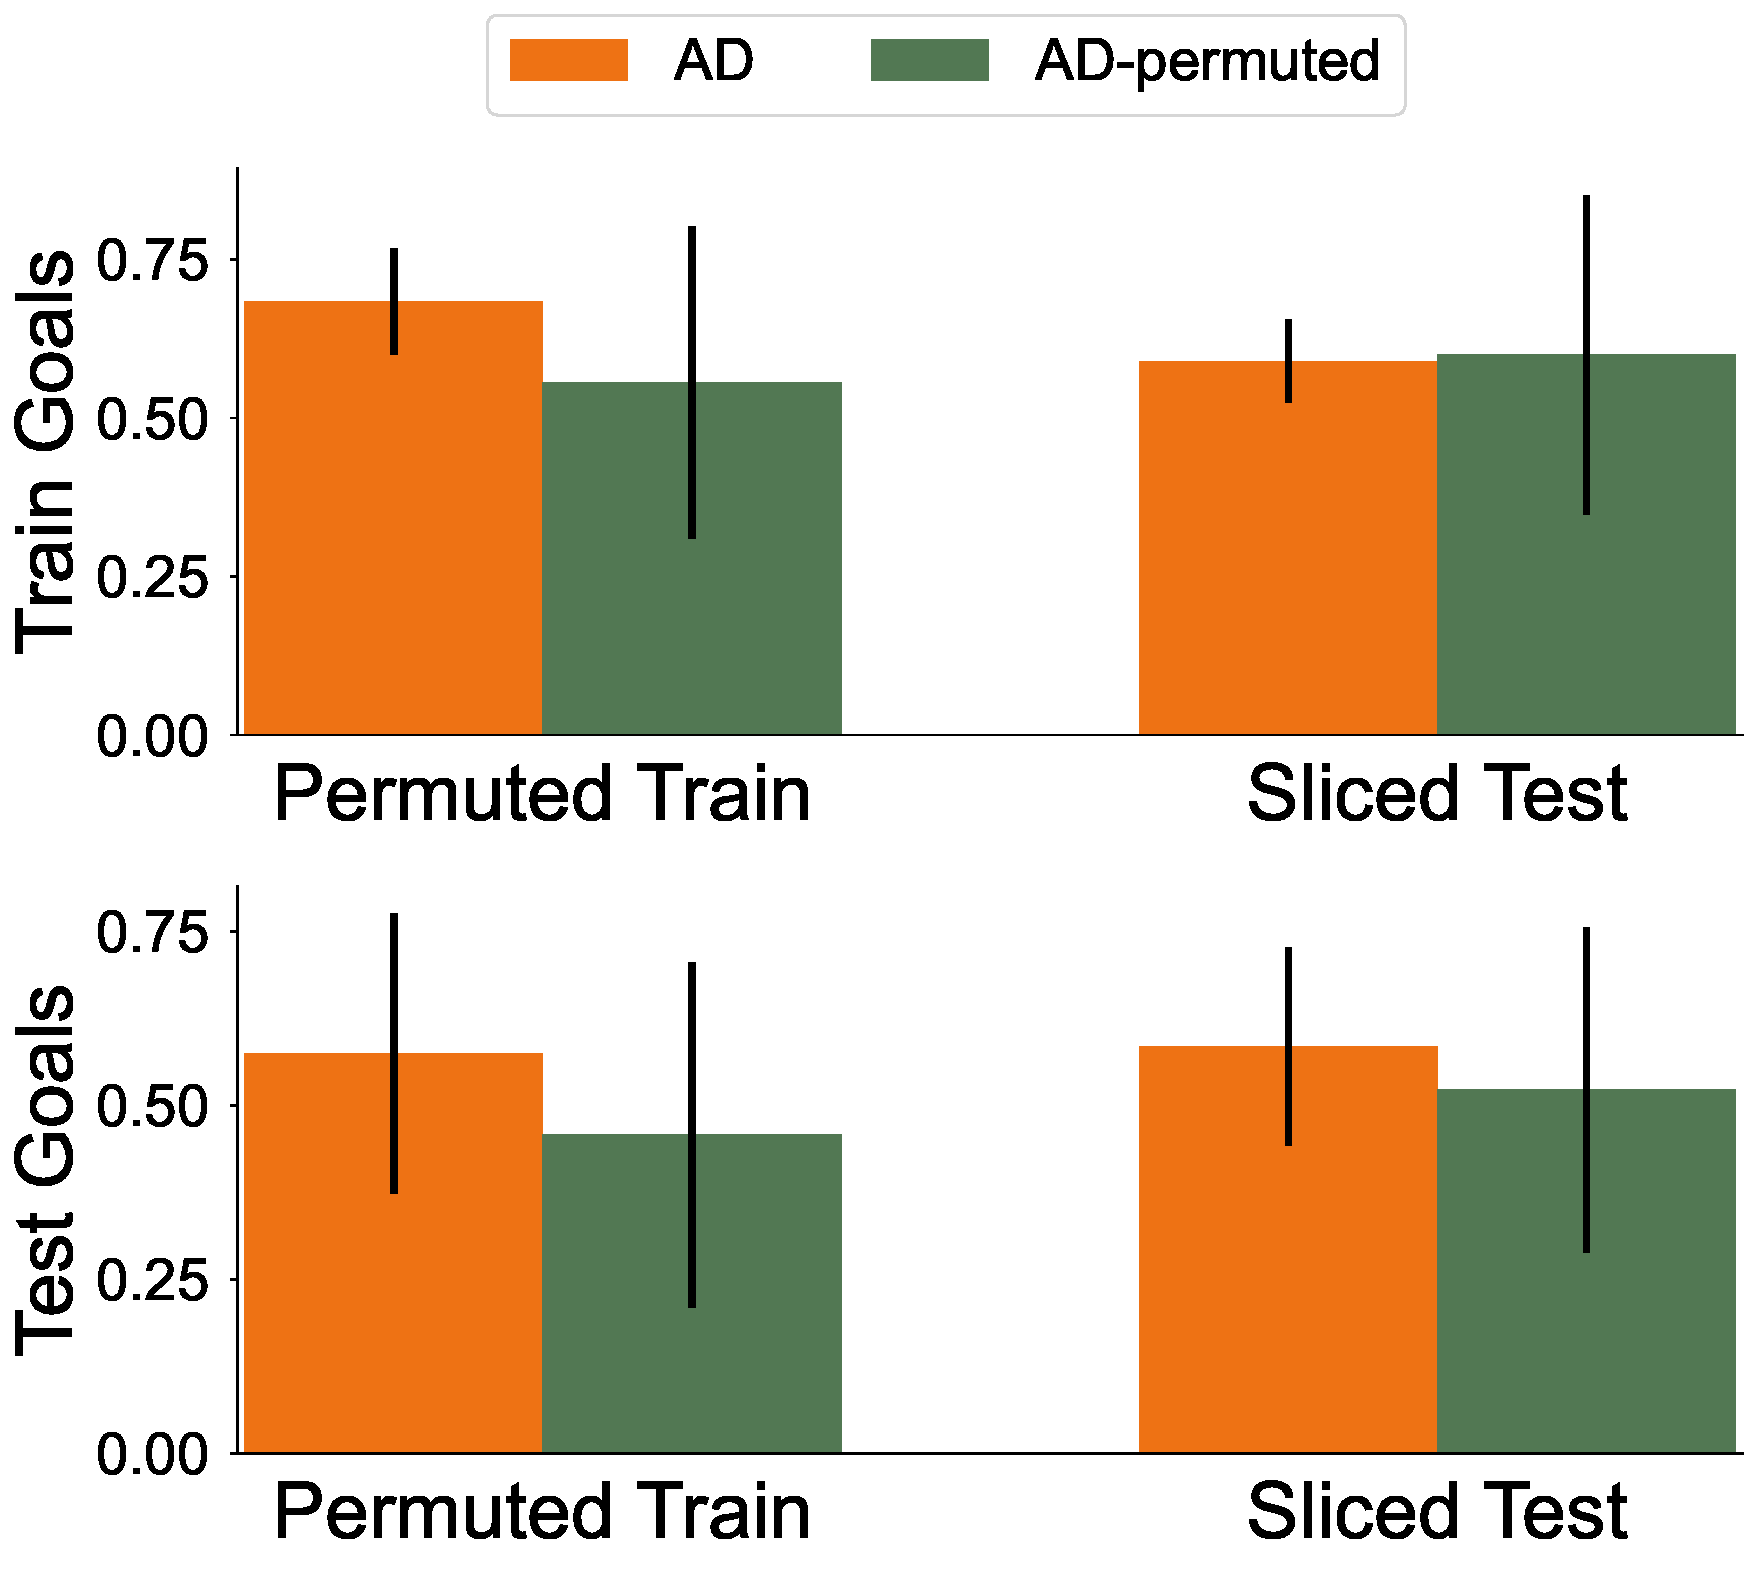
\includegraphics[width=0.7\columnwidth]{images/gridworld_vanilla_perm.pdf}
%     \caption{\textbf{AD Performance on Permuted Actions:} We evaluated AD's ability to adapt to action sets with varied semantics by training it on a permuted dataset. Except of this, the training and testing are the same as in vanilla setting and can be found in \Cref{eval:gridworld}. Contrary to expectations, this tailored training did not enhance performance when compared to the AD model trained on standard datasets.}
%     \label{fig:gridworld_vanilla_perm}
% \end{figure}
